\documentclass{article}

\usepackage{times}
\usepackage{amsthm}
\usepackage{amsmath}
\usepackage{amssymb}
\usepackage{listings}

\usepackage[font=footnotesize]{caption}
\usepackage[font=footnotesize]{subcaption}
\usepackage[pdftex]{graphicx}
\usepackage{wrapfig}
\usepackage{epstopdf}
\usepackage[american]{babel}
\usepackage{url}
\usepackage{color}
\usepackage{xspace}
\usepackage{float}
\usepackage{tabularx}
\usepackage{multirow}
\usepackage{alltt}
\usepackage{multicol}
\usepackage{blindtext}
\usepackage{scrextend}
\usepackage{geometry}
\usepackage{hyperref}
\addtokomafont{labelinglabel}{\sffamily}

\definecolor{dkgreen}{rgb}{0,0.6,0}
\definecolor{gray}{rgb}{0.5,0.5,0.5}
\definecolor{mauve}{rgb}{0.58,0,0.82}

\lstset{frame=tb,
	language=R,
	aboveskip=3mm,
	belowskip=3mm,
	showstringspaces=false,
	columns=flexible,
	basicstyle={\small\ttfamily},
	numbers=none,
	numberstyle=\tiny\color{gray},
	keywordstyle=\color{blue},
	commentstyle=\color{dkgreen},
	stringstyle=\color{mauve},
	breaklines=true,
	breakatwhitespace=true,
	tabsize=3
}

\usepackage{algorithmic}
\renewcommand{\algorithmiccomment}[1]{// #1} % Brackets are confused with the sets
\usepackage{algorithm} % For counting chapters
\algsetup{linenosize=\scriptsize}
\xspaceaddexceptions{=}
\xspaceaddexceptions{\}}
\xspaceaddexceptions{\in}

\geometry{margin=0.75in}

% A set depicted with bold:
\newcommand{\set}[1]{\ensuremath{\mathbf{#1}}\xspace}

% The elements of a set:
\newcommand{\elements}[3]{\ensuremath{\{#1_{#2},...,#1_{#3}\}}\xspace} 

%The cardinality of a given set belonging somewhere:
\newcommand{\cardinality}[2]{\ensuremath{|\set{#1}_{#2}|}\xspace} 		

% A mathematical unit:
\newcommand{\unit}[1]{\ensuremath{\mathrm{#1}}\xspace} 	

\DeclareMathOperator*{\argmin}{arg\,min}

\newtheorem{definition}{Definition}

% correct bad hyphenation here
\hyphenation{}

\title{An analysis of high impact traffic collisions in Toronto}
\author{Christopher Salahub}

\begin{document}
\maketitle

\section{Issue} \label{sec:Issue}

The
\href{http://data.torontopolice.on.ca/datasets/ksi?geometry=-80.249%2C43.55%2C-78.515%2C43.897&selectedAttribute=IMPACTYPE}{\textit{KSI}}
data set provided by the Toronto Police Service displays detailed characteristics of all traffic collision events in which
individuals in Toronto were either seriously injured or killed between 2007 and 2017. While such data is useful to illuminate the past in its own right,
it also provides the opportunity to find useful insights which can assist in the present management of resources and can direct future public education

\section{Data} \label{sec:Data}

While the KSI data set is quite thorough in detailing incidents, it conspicuously lacks accurate weather data. Such data may prove
useful in a predictive or educational setting, and so weather data was extracted from the Government of Canada
\href{http://climate.weather.gc.ca/index_e.html}{\textit{climate data website}}. This extraction was completed using the batch
\href{ftp://ftp.tor.ec.gc.ca/Pub/Get_More_Data_Plus_de_donnees/Readme.txt}{\textit{data extraction API}} and a custom function coded in the \texttt{R} programming language (see the \texttt{ClimatePull} function in the code in \ref{appendix}). This data is recorded on
an hourly basis at many stations across Canada, however the only station which had hourly data for the entirety of the KSI date
range was Toronto City Centre. Fortunately, this weather station is centrally located in the KSI data (see
\ref{appendix}.\ref{fig:weatherstation}). Unfortunately, it was rather incomplete. The wind speed, wind direction, visibility, humidex, wind
chill, and weather variables were all completely uninformative, and so only temperature, pressure, humidity, and dew point data
was used in analysis.

The KSI data, downloaded in CSV format from the Toronto Police Service (TPS) website, was more complete, but even this data had
missing and uninformative entries. Blank fields were highly prevalent in the data, and the expected interpretation of these blank entries
was not clear. As a result, these entries were assumed to be uninformative, and were categorized as ``Other''. Particularly specific
values in any field were generalized and combined into general categories (e.g. ``Laneway'' categorized as ``Local'') under the
assumption that this extra information was simply not recorded in most cases. Finally, some unique categories were single
occurrences over the entire ten year window, and so did not form a good inferential basis for policy decisions. These were also
categorized as ``Other'' (e.g. the value of ``Spilled liquid'' for the road surface condition). This data was analyzed on two
separate scales: first on the scale of individuals as recorded in the original data, and second on the scale of collision events as given by the \texttt{ACCNUM} variable.

One severe limitation of the KSI data is the lack of normalizing traffic counts. In a predictive or classification sense, the
entirety of this data set consists of ``positive'' results. Put in other words: one cannot identify the exceptional circumstances
which lead to severe collisions without seeing the typical data that serves as the non-exceptional baseline. The overall
consistency of the data across the temporal and spatial window sampled supports this notion. An attempt to extract data from Toronto's
Open Data portal
(\href{https://www.toronto.ca/city-government/data-research-maps/open-data/open-data-catalogue/transportation/#7c8e7c62-7630-8b0f-43ed-a2dfe24aadc9}{\textit{traffic
    and pedestrian volumes}}) was pursued, but time constraints prevented that analysis from coming to fruition.

\section{Methods} \label{sec:methods}

Visual methods were utilized to explore the data before any models were fit. This was not only enlightening, but has created a series of communicative plots which can be used to inspire future investigations and reveal data patterns. Scatterplots were used to explore the continuous variables, while the categorical
variables were analyzed using mosaic plots. These plots allocate visual area within set plot boundaries proportionally to the cell
magnitudes in a contingency table. They are incredibly useful visual tools to detect dependencies between categorical
variables. The \texttt{R} implementation additionally shades those values which are statistically significant in a Pearson chi-square test
of independence to make this detection easier. The \texttt{R} functions \texttt{plot} and \texttt{mosaicplot} were used for scatterplots and mosaic plots
respectively. A custom function, \texttt{panelPlot}, was designed to display categorically filtered levels of continuous
variables.

In order to remove redundancies in the weather data, principal component analysis was performed in the pre-processing
stages. Principal component analysis aims to reduce the dimensionality of a data set without reducing the information by finding
the optimal projection vectors for the data. The result of this principal component analysis -- performed using \texttt{princomp}
in \texttt{R} --  was a reduction of the four weather variables to only two principal components, which together still explained
roughly 83\% of the variation in the weather data.

Finally, a series of mixed logistic regression models was fit using \texttt{lme4} in \texttt{R} in an attempt to more precisely
identify the features predictive of fatal accidents. Their natural regularization and protection from over-fitting, as well as the
flexibility to handle crossed and nested fixed and random covariates, motivated this choice. Given more time, this analysis would
continue. Currently, the analysis was limited to mixed models on the collision event scale with random effects for only the wards
and TPS divisions, but analysis on the scale of individuals involved in collision events, with the collision event treated as a
random effect itself, could prove incredibly fruitful. Indeed, such analysis has the potential to reveal which of the collision
events in the data are ``unusually'' severe.

\section{Analysis} \label{sec:analysis}

The first visual investigation was a simple spatial plot of collisions on the scale of unique collision incidents, coloured by
fatality. The plot, Figure, \ref{appendix}.\ref{fig:fatalitymap}, shows no obvious spatial patterns to the collisions by severity; collision events are spread about Toronto roughly evenly at all severity levels. Splitting by impact type, however, reveals more interesting
spatial relations. The output of \texttt{panelPlot} applied to this data, with additional colours added by TPS division, is shown
in Figure \ref{appendix}.\ref{fig:impactpanel}. Note that the map background (previously provided by the \texttt{ggmap} package in
\texttt{R}) has been dropped in these panels, in order to bring greater focus to the points.

Several patterns are worthy of note in this plot. The primary, and most striking, is the high prevalence of pedestrian collisions
in this data set. The panel displaying the locations of the pedestrian collisions has far more points, placed far more regularly
across the window, than any other category. In fact, 44\% of all collisions in this data set are pedestrian collisions, more than
three times the next most common category, turning movements, at 13\%. This suggests that education and investigation into safer
pedestrian street designs could have a significant impact on the occurrence of severe collisions. The universality of this high pedestrian impact volume suggests
that such efforts must be pursued across every TPS division.

Not all divisions should expect each impact type equally, however, despite the dominance of pedestrian collisions in the data. Figure
\ref{appendix}.\ref{fig:impactdivision} displays the unique impact type frequency of each TPS division. Note that some of these results
are clear in Figure \ref{appendix}.\ref{fig:impactpanel}, such as the increased burden of bicyclist collisions for D14. These
results provide a more nuanced perspective of which initiatives to counter extreme collisions deserve the most attention in each
division.

Single marginal temporal investigations showed stable, if uninformative, patterns in the collision data, as shown in Figure
\ref{appendix}.\ref{fig:timedayind}. While there is a clear visible gap between four and six in the morning, the fatal collisions
do not seem to cluster around any particular times. Indeed, even the increases in point density that might be expected near rush hour do not seem
to be present in this plot. This suggests that effective response to severe collisions cannot assume that high volume traffic times
are at higher risk of a severe accident, as that pattern is not present in the historical data.

On the other hand, temporal investigations which incorporated the TPS divisions gave very informative results. Figure
\ref{appendix}.\ref{fig:divisionhour}. This plot shows markedly different patterns for each of the divisions, and given the lack
of trend seen year-to-year in Figure \ref{appendix}.\ref{fig:timedayind}, these patterns are likely stable. The mosaic plot display of
this data is also exceptionally useful, because it makes planning for logistical requirements simple. One must simply find the desired
division on the top row, scan down the corresponding column for blue squares, and plan for extra rapid response personnel accordingly, as these
squares correspond to the hours with abnormally high collision frequencies.

Further plots and model fitting failed to produce results as immediately useful as those outlined above. While the code below
contains many more combinations of variable plots than those seen here, the results presented in this report are more insightful
than any others. The model fitting, in particular, failed to produce any interesting results. As outlined in Section
\ref{sec:methods}, however, this is mostly a reflection of a lack of time spent investigating this data. Another promising avenue of
investigation is the prediction of road conditions using the synthesized weather principal components, as a plot of these
components coloured by road surface conditions (see Figure \ref{appendix}.\ref{fig:roadcondweather}) showed reasonably good
separation of road conditions.

\section{Results}

The primary results of this investigation and the automated aggregation of collision data by unique event are the profiles of the
different TPS divisions. These profiles can provide guidance to division leaders as to the hours which will require the
greatest numbers of staff ready to respond to serious calls, as well as suggesting particular local public education efforts. A critical
observation of this analysis is that almost half of fatal collisions involve pedestrians, and that indicates public education and
pedestrian safety investigation are critical.

\clearpage

\section{Appendix} \label{appendix}

\begin{figure}[!h]
	\begin{center}
		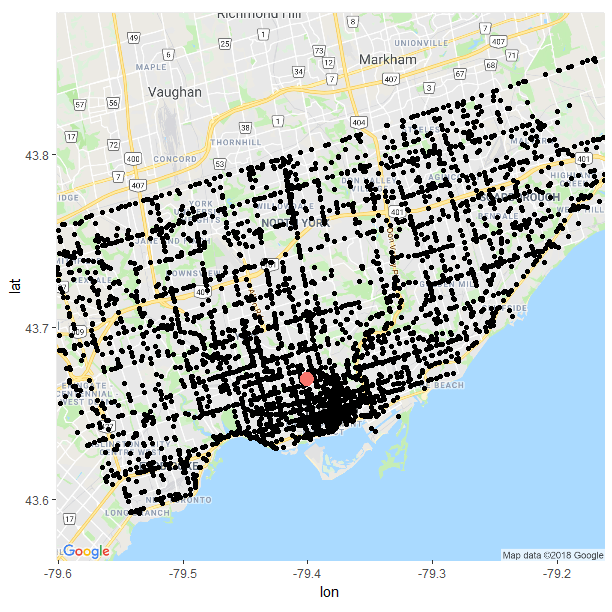
\includegraphics[scale=0.75]{WeatStat}
		\caption{The weather station (large red point) and observed collisions}
		\label{fig:weatherstation}
	\end{center}
\end{figure}

\begin{figure}[!h]
	\begin{center}
		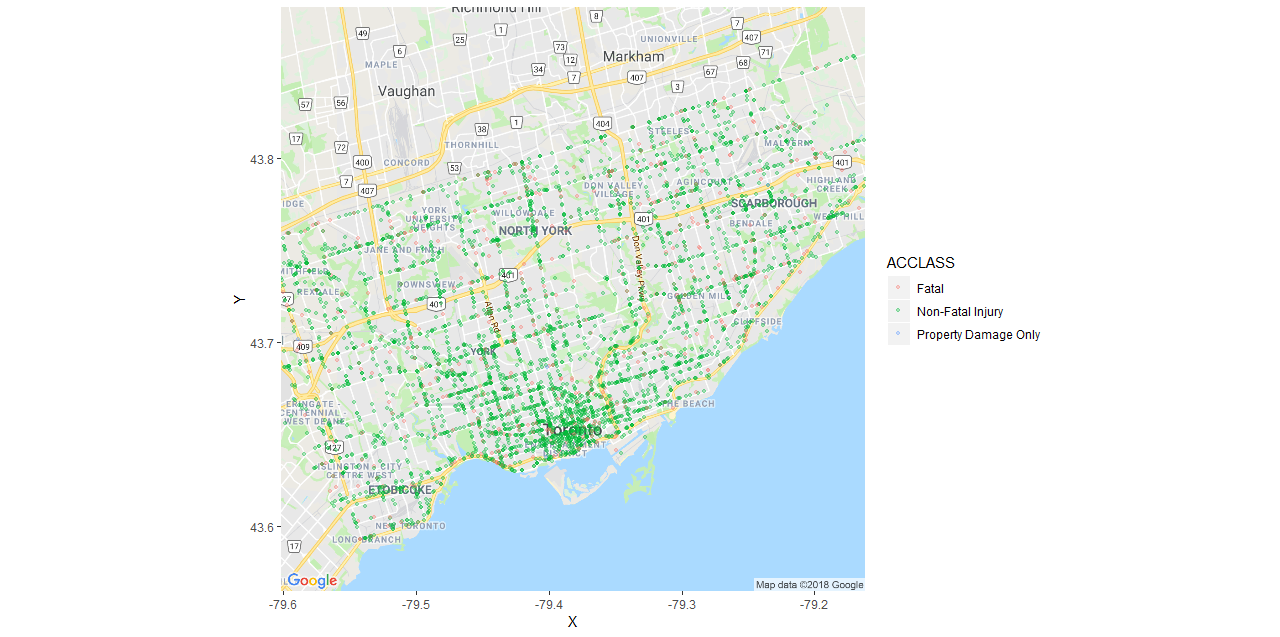
\includegraphics[scale = 0.5]{FatalityMap}
		\caption{Collisions coloured by severity of outcome}
		\label{fig:fatalitymap}
	\end{center}
\end{figure}

\begin{figure}[!h]
	\begin{center}
		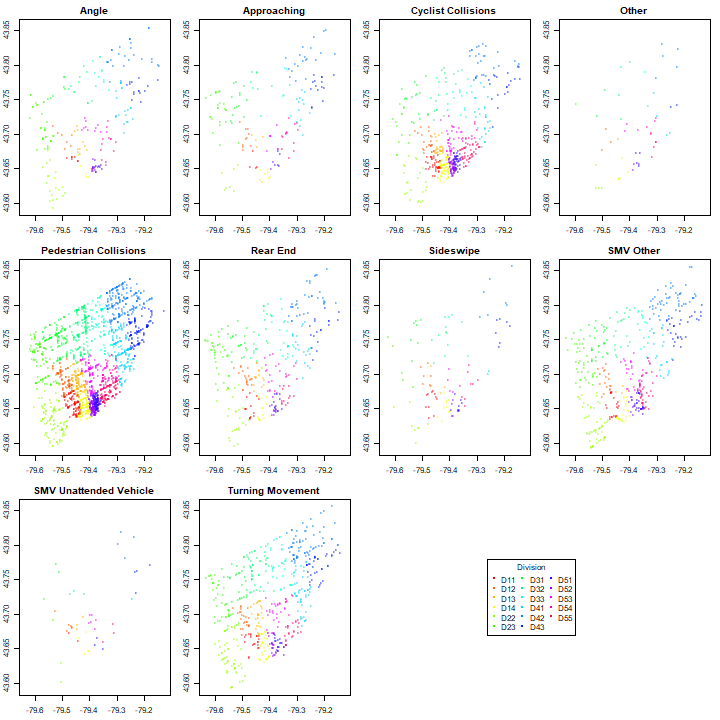
\includegraphics[scale = 0.75]{impactPanel}
		\caption{Collision locations, panelled by impact type, and coloured by the TPS division that responded}
		\label{fig:impactpanel}
	\end{center}
\end{figure}

\begin{figure}[!h]
	\begin{center}
		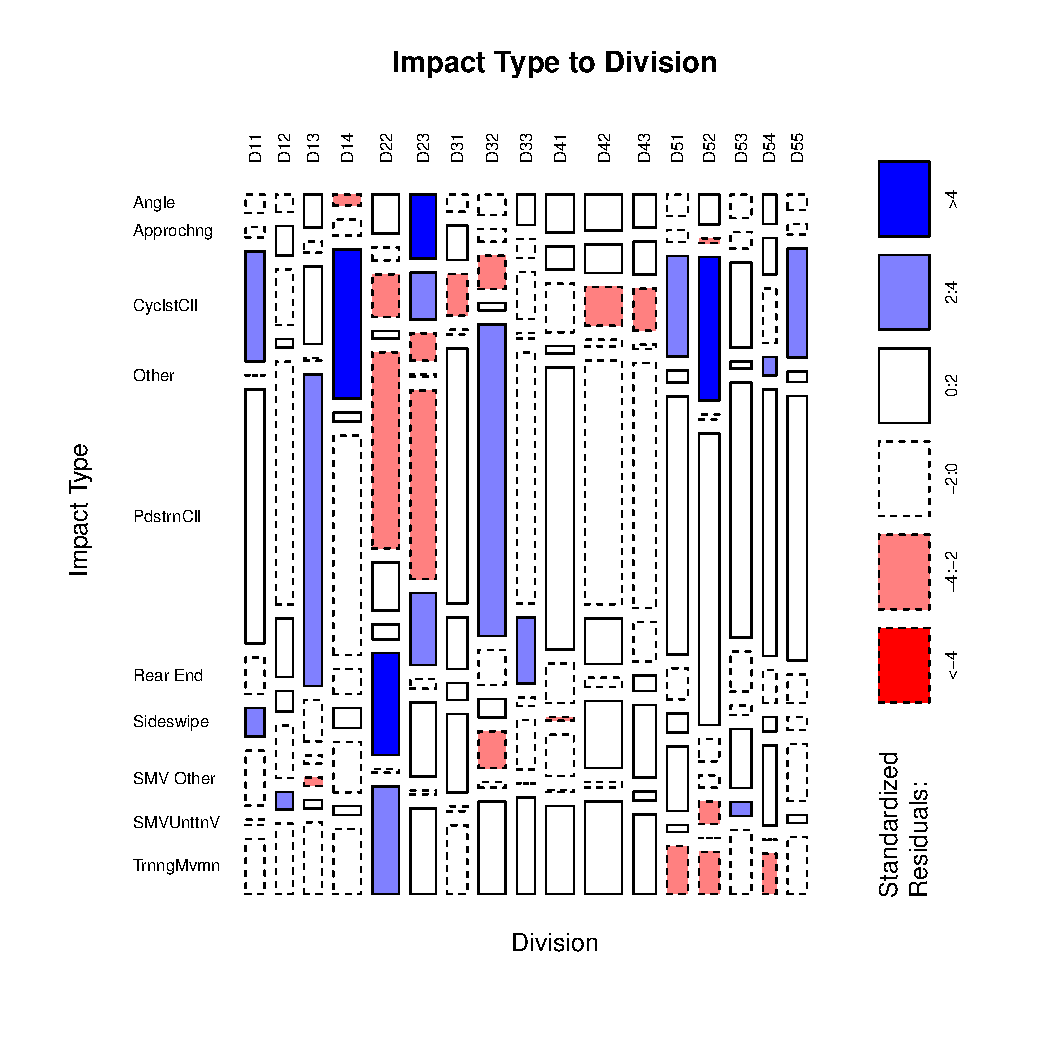
\includegraphics[scale = 1]{impactDivision}
		\caption{Impact type by TPS division responding, with statistically significant differences shaded}
		\label{fig:impactdivision}
	\end{center}
\end{figure}

\begin{figure}[!h]
	\begin{center}
		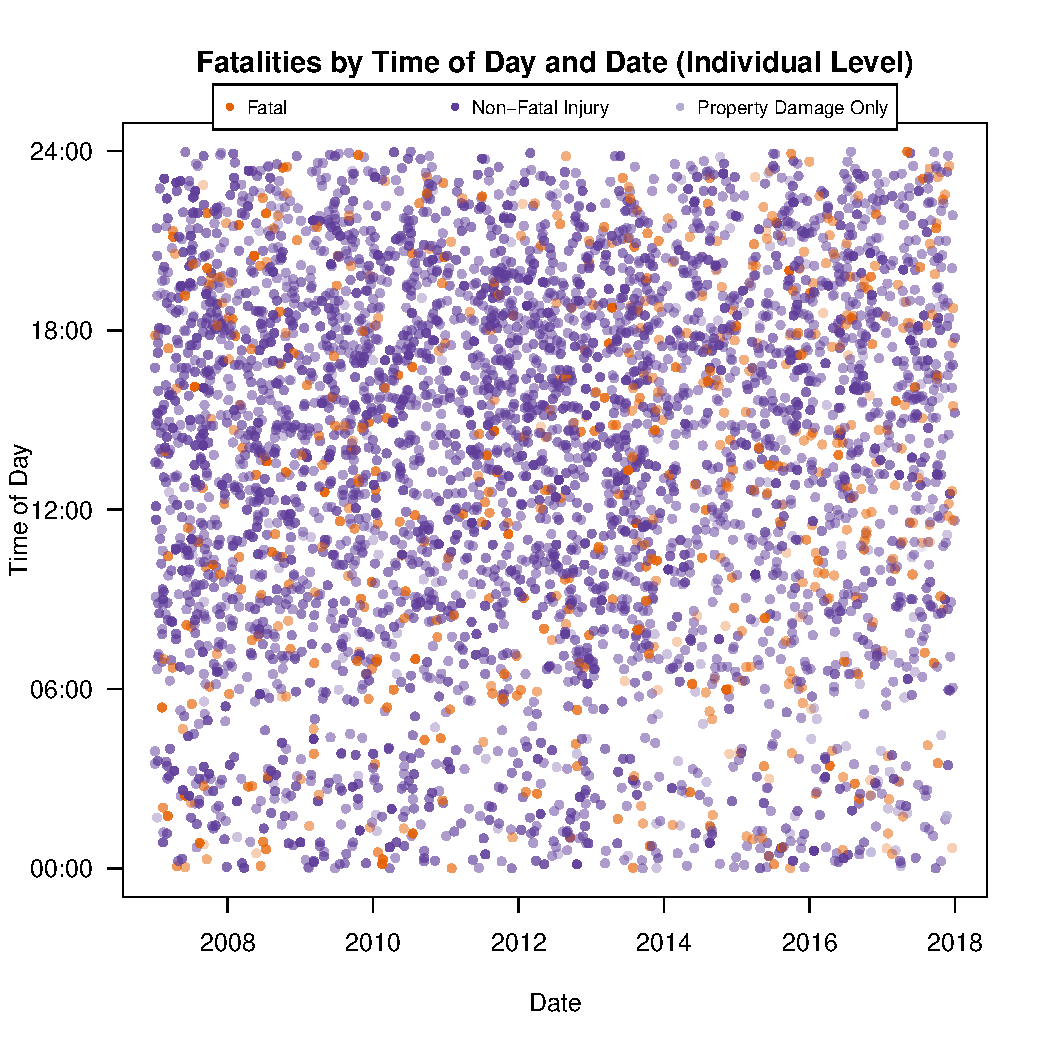
\includegraphics[scale = 1]{timedayind}
		\caption{Collision severity by time of day and date, displayed on the involved individual scale}
		\label{fig:timedayind}
	\end{center}
\end{figure}

\begin{figure}[!h]
	\begin{center}
		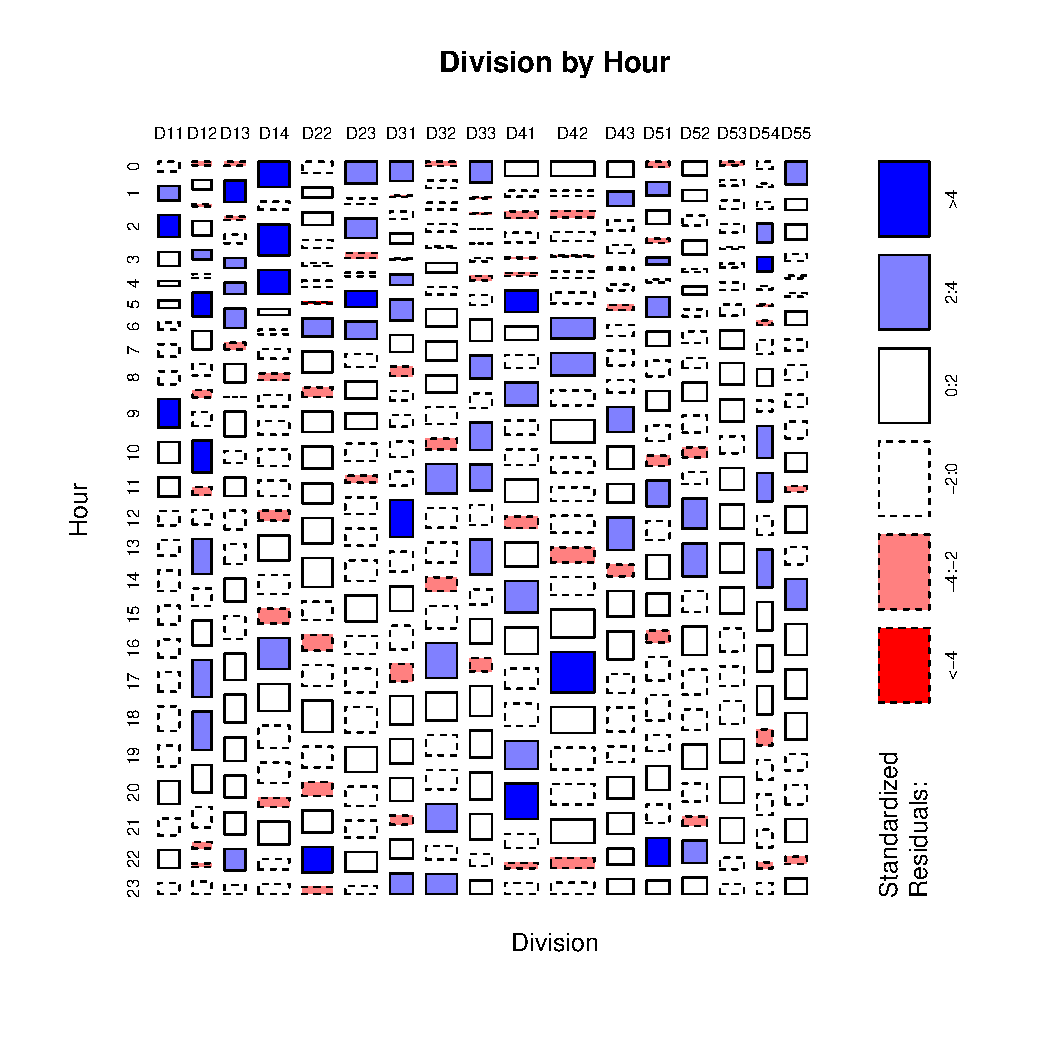
\includegraphics[scale = 1]{divisionhour}
		\caption{Mosaic plot of TPS division and hour, showing very different time profiles for each division}
		\label{fig:divisionhour}
	\end{center}
\end{figure}

\begin{figure}[!h]
	\begin{center}
		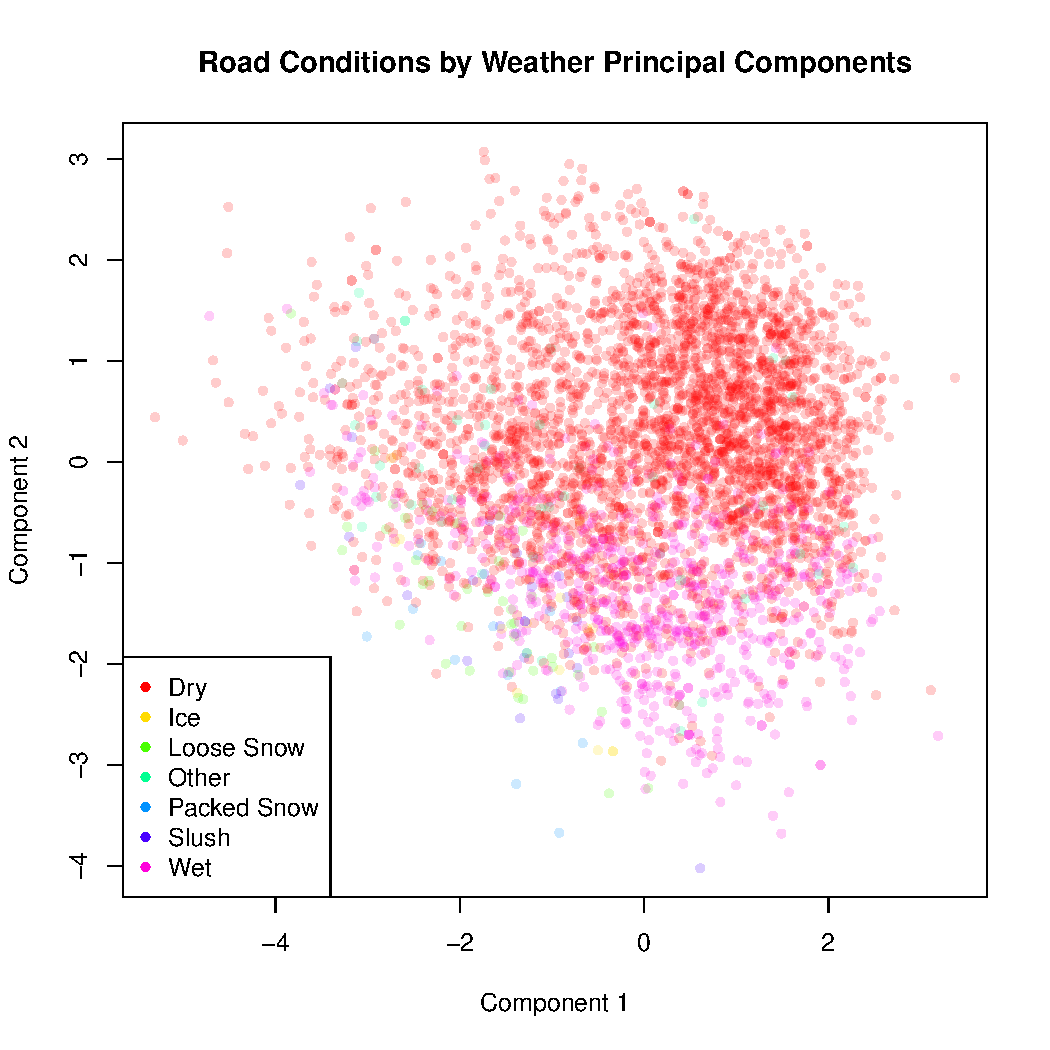
\includegraphics[scale = 1]{roadcondweather}
		\caption{Plot of weather principal components coloured by road conditions, note the separation of the different colours of points}
		\label{fig:roadcondweather}
	\end{center}
\end{figure}


\end{document}
